\documentclass[12pt]{article}
\usepackage[a4paper, margin=1.5cm]{geometry}

\usepackage{multicol}
\usepackage{lipsum}
\usepackage{tikz}
\usepackage{graphicx}

% for the fillspacewithplaceholder command
\newlength{\remainingheight}%

\newcommand{\fillspacewithplaceholder}[1][90]{%
  \par % force vertical mode
  \setlength{\remainingheight}{\dimexpr (\pagegoal-\pagetotal)*#1/100\relax}%
  \begin{center}%
  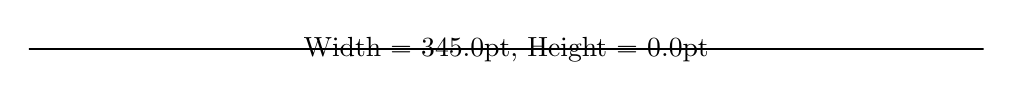
\begin{tikzpicture}%
    % Draw rectangle using stored height
    \draw[thick] (0,0) rectangle (\columnwidth,\remainingheight);%
    % Place node in the center
    \node at (0.5\columnwidth,0.5\remainingheight) {Width = \the\columnwidth, Height = \the\remainingheight};%
  \end{tikzpicture}%
  \end{center}%
}

\begin{document}
\section*{Single Column, A Little text.}
\lipsum[1]
\fillspacewithplaceholder
\newpage

\section*{Single Column, some text.}
\lipsum[1-4]
\fillspacewithplaceholder
\newpage

\section*{Single Column, LOADS of text.}
\lipsum[1-8]
\fillspacewithplaceholder
\newpage

\section*{Dual Column, "good" amount of text.}
\begin{multicols}{2}
\lipsum[1-5]
\fillspacewithplaceholder
\end{multicols}
\newpage

\section*{Dual Column, "good" amount of text - Actual Image.}
\begin{multicols}{2}
\lipsum[1-5]

\includegraphics{DualColLipsum1-5.png}%
\end{multicols}
\newpage

\section*{File Interactions...}

\IfFileExists{testImageL.png}{%
  \includegraphics[width=0.5\textwidth]{testImageL.png}%
}{%
  \textbf{Image is missing!}%
}

\IfFileExists{nonExistantImage.png}{%
  \includegraphics[width=0.5\textwidth]{nonExistantImage.png}%
}{%
  \textbf{Image is missing!}%
}


\section*{File Interactions...}
\begin{multicols}{2}
\lipsum[1-3]
\IfFileExists{nonExistantImage.png}{%
  \includegraphics[width=0.5\textwidth]{nonExistantImage.png}%
}{%
  \fillspacewithplaceholder
}
\end{multicols}
\newpage



\end{document}